Today we will discuss fermionic Yukawa theory. Before, we looked at Yukawa theory in a simplified scalar case. However, nucleons are really fermions. The interactions between fermions and a scalar particle are governed by the Yukawa interaction,
$$\cL=\frac{1}{2}\p_\mu \phi \p^\mu \phi -\underbrace{\frac{\mu^2}{2}\phi^2}_{\text{scalar mass}} +\bar \psi (i\slashed{\p}-m)\psi -\underbrace{\lambda \phi \bar \psi \psi}_{\text{Yukawa interaction}}.$$
From the kinetic terms, we see that $[\phi]=1$ and $[\psi]=[\bar \psi]=3/2,$ which is a bit unusual. We conclude that $[\lambda]=0$ which means that this coupling is \emph{marginal}.

Let us consider again the process of nucleon-nucleon scattering, $\psi\psi\to \psi\psi.$ Now we must keep track of spin indices as well as momentum. Our initial state is a two-particle state
$$\ket{i}=\sqrt{2E_p}\sqrt{2E_q}b_{\vec p}^{s\dagger}b_{\vec q}^{r\dagger}\ket{0}$$
and our final state is similar,
$$\ket{f}=\sqrt{2E_{p'}}\sqrt{2E_{q'}}b_{\vec p'}^{s'\dagger}b_{\vec q'}^{'r\dagger}\ket{0}$$
As before, we will disregard the $O(\lambda^0)$ term where the particles do not interact, and there is no $O(\lambda)$ term as in the scalar case. Therefore the leading order interesting behavior is the $O(\lambda^2)$ term:
\begin{equation}
    \bra{f}(S-1)\ket{i}=\bra{f}\frac{(-i\lambda)^2}{2!}\int d^4 x_1 d^4 x_2 T\left[\bar \psi(x_1)\psi(x_1)\phi(x_1)\bar \psi(x_2)\psi(x_2)\phi(x_2)\right]\ket{i}.
\end{equation}
All fields are in the interaction picture as usual. We'll use Wick's theorem to compute the time ordering. The contribution to the scattering then comes from the contraction
$$:\bar \psi(x_1)\psi(x_1)\bar \psi(x_2)\psi(x_2):\overbrace{\phi(x_2)\phi(x_1)}.$$
Thus the $\psi$s will annihilate the $\ket{i}$ and the $\bar \psi$s will create $\bra{f}.$ In order to put the normal-ordered bit in the right order, we must anticommute $\bar \psi(x_2)$ past $\psi(x_1)$, picking up a sign flip for our trouble. We therefore get the interaction
\begin{align*}
    I&\equiv :\bar \psi_\alpha(x_1)\psi_\alpha(x_1)\bar \psi_\beta(x_2)\psi_\beta(x_2): b_{\vec p}^{s\dagger} b_{\vec q}^{r\dagger}\ket{0}\\
    &=- \int \frac{d^3k_1 d^3k_2}{(2\pi)^6 2\sqrt{E_{k_1} E_{k_2}}} \left[\bar \psi_\alpha(x_1) U_{\vec k_1,\a}^m\right] \left[\bar\psi_\beta (x_2) U_{\vec k_2,\beta}^n\right] e^{-i(k_1x_1+k_2x_2)}b_{\vec k_1}^m b_{\vec k_2}^n b_{\vec p}^{s\dagger} b_{\vec q}^{r\dagger}\ket{0}.
\end{align*}
Here, the $U$s are the planar wave solutions from before, and the square bracket means that we contract over the four spinor indices. The other terms i the expansion go to zero because they have either $\bra{0}c^\dagger=0$ or $c\ket{0}=0.$ Looking at the creation and annihilation operators, we can rewrite as
\begin{align*}
    b_{\vec k_1}^m b_{\vec k_2}^n b_{\vec p}^{s\dagger}b_{\vec q}^{r\dagger}\ket{0} &=(b_{\vec k_1}^m \set{b_{\vec k_2}^n b_{\vec p}^{s\dagger}}b_{\vec q}^{r\dagger}
    -b_{\vec k_1}^m b_{\vec p}^{s\dagger} \set{b_{\vec k_2}^{n}b_{\vec q}^{r\dagger}})\ket{0}\\
    &=(\set{b_{\vec k_1}^m b_{\vec q}^{r\dagger}}\set{b_{\vec k_2}^n b_{\vec p}^{s\dagger}}
    -\set{b_{\vec k_1}^m b_{\vec p}^{s\dagger}} \set{b_{\vec k_2}^{n}b_{\vec q}^{r\dagger}})\ket{0},
\end{align*}
where we have used the fact that annihilation operators kill the vacuum state and anticommutators are just c-numbers. Thus this whole expression becomes delta functions,
$$(2\pi)^6 [\delta^3 (\vec k_2 -\vec p)\delta^3 (\vec k_1-\vec q)\delta^{ns}\delta^{mr}-\delta^3 (\vec k_1-\vec p) \delta^3(\vec k_2-\vec q)\delta^{ms}\delta^{nr}]\ket{0}.$$
Hence $I$ simplifies somewhat to
$$I=-\frac{1}{2\sqrt{E_pE_q}}\left\{[\bar \psi(x_1)U_{\vec q}^r][\bar\psi(x_2)U_{\vec p}^s] e^{-i(q\cdot x_1 +p\cdot x_2)}
-[\bar \psi(x_1)U_{\vec p}^s][\bar\psi(x_2)U_{\vec q}^r] e^{-i(p\cdot x_1 +q\cdot x_2)}\right\}\ket{0}.$$
We still need to apply the final state to get
$$-\frac{2\sqrt{2 E_{p'}E_{q'}}}{2\sqrt{E_pE_q}} \bra{0}b_{\vec q'}^{r'}b_{\vec p'}^{s'}
\left\{[\bar \psi(x_1)U_{\vec q}^r][\bar\psi(x_2)U_{\vec p}^s] e^{-i(q\cdot x_1 +p\cdot x_2)}
-[\bar \psi(x_1)U_{\vec p}^s][\bar\psi(x_2)U_{\vec q}^r] e^{-i(p\cdot x_1 +q\cdot x_2)}\right\}\ket{0}.$$
From here, we pass to the integral representation, writing
$$-\frac{2\sqrt{2 E_{p'}E_{q'}}}{2\sqrt{E_pE_q}} \bra{0}\left[ \int \frac{d^3k_1 d^3k_2}{2\sqrt{E_{k_1}E_{k_2}}(2\pi)^6} b_{\vec q'}^{r'}b_{\vec p}^{s'}[\bar U_{k_1}^m U_{\vec q}^r] b_{\vec k_1}^{m\dagger} b_{\vec k_2}^{n\dagger} [\bar U_{k_2^n}u_{\vec p}^s] e^{i(k_1x_1+k_2x_2)-i(q\cdot x_1 +p\cdot x_2)}-\ldots\right]$$
where the $\ldots$ indicates a similar term with $p$ and $q$ switched, $r$ and $s$ switched.
But the $b$s pair up nicely to give us delta functions:
$$b_{\vec q'}^{r'}b_{\vec p}^{s'} b_{\vec k_1}^{m\dagger} b_{\vec k_2}^{n\dagger}=(2\pi^6)\bra{0}(\delta^{s'm}\delta^{r'n}\delta^3(\vec p- \vec k_1)\delta^3(\vec q'-\vec k_2)-\ldots)$$
where $\ldots$ is the same with $m,n$ switched and $\vec k_1,\vec k_2$ switched. After applying delta functions (check the Tong notes for this) the expression cleans up in the same way that the Feynman diagrams would have shown us, but keeping track of spins. Writing $\bra{f}(S-1)\ket{i}=iM(2\pi)^4 \delta^4(p+q-p'-q'),$ we get
\begin{equation}
    M=-(-i\lambda)^2 \left\{ \frac{[\bar U_{\vec p'}^{s'} U_q^r][\bar U_{\vec q'}^{r'}u_{\vec p}^s]}{(q'-p)^2-\mu^2+i\epsilon}
    - \frac{[\bar u_{\vec q'}^{r'}U_{\vec q}^r][\bar U_{\vec p'}^{s'} U_{\vec p}^s]}{(p'-p)^2-\mu^2+i\epsilon}\right\}.
\end{equation}

That was a lot of work. What can Feynman tell us about this matrix element? We have some momentum space Feynman rules for fermion amplitudes. They are as follows. 
\begin{itemize}
    \item Dirac fermions preserve fermion number, so the arrows must not clash (e.g. no two arrows into a vertex).
    \item Incoming fermions get a momentum and a spinor index, $U_{\vec p}^s$. Outgoing fermions get $\bar U_{\vec p}^s$ instead.
    \item Incoming antifermions get $\bar v_{\vec p}^s$ and outgoing antifermions, $v_{\vec p}^s$.
    \item We impose 4-momentum conservation at each vertex.
    \item Each three-point vertex with a dashed line (the scalar) gets a factor of $(-i\lambda)$.
    \item Internal lines for $\psi$s with spinor indices $\alpha$ going to $\beta$ get propagators $$\frac{i(\slashed{p}+m)_{\beta\alpha}}{p^2-m^2+i\epsilon},$$
    where these $\alpha,\beta$ indices are contracted at vertices with other propagators or with external spinors. (The indices are contracted in the opposite direction to the fermion number arrows.)
\end{itemize}

\begin{figure}
    \centering
    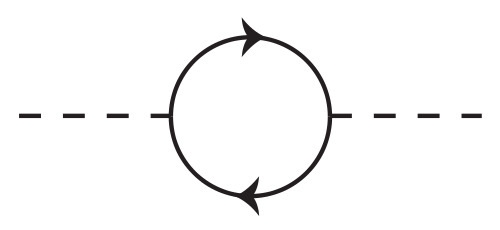
\includegraphics[width=0.5\textwidth]{2018/11/20181117_oneloop.png}
    \caption{The closed fermion loop diagram. Image from \href{https://commons.wikimedia.org/wiki/File:One-loop-diagram.svg}{Wikipedia}.}
    \label{fig:oneloop}
\end{figure}
For example, for the closed fermion loop in Fig. \ref{fig:oneloop} we get an amplitude which goes as
$$-\overbrace{\bar \psi_\alpha(x) \overbrace{\psi_\alpha(x) \bar \psi_\beta(y)} \psi_\beta(y)}=-\overbrace{\psi_\beta(y) \bar \psi_\alpha(x)}\overbrace{\psi_\alpha(x)\bar \psi_\beta(y)}.$$
So we get an additional minus sign for a fermion loop, as well as the usual $d^4k/(2\pi)^4$ and fermion propagators.